\chapter{Results}
\label{chap:results}

As stated in Chapter~\ref{chap:methodology}, it is not possible to realize an
extensive accuracy study due to the absence of an events dataset.
However, this chapter presents illustrative examples when the proposed pipeline
was applied to real data.

It was considered 8 months of measurements, from may to december 2016.
This data was then divided in batches of 10 days, and for each batch,
a complete analysis was executed.

Considering all batches, after the End-Users Filtering procedure,
the number of target clients varied from X to X, through the X servers.
Figure~\ref{fig:path_length_distribution} presents a histogram of the path
length, in number of edges, between zero indegree vertexes and the server
vertex. Figure~\ref{fig:indegree_distribution} show the indegree distribution
of the user-groups.

For all cases, the time series were preprocessed with a median filter.
The change points were detected through the optimization model described in
Chapter~\ref{chap:change_point_detection}.
For each QoS metric, the algorithms' hyperparameters were manually selected.
It was opted by conservative values, in order to avoid change points that,
through a visual inspection, may be arguably not related to a network event.
Those algorithms choices were guided by two facts.
First, through a empirical visual analysis,
it was verified their reasonable perfomance with real data.
Also, the impact of their hyperparameters can be easily interpreted, which is
an important feature to manual tuning.

The event detection can be interpreted as a binary classification problem, in
which events represent the positive class.
Then, Section~\ref{sec:possible_true_positive_examples} presents some
possible true positive cases.
Also, it is illustrated the reasoning behind the events localization process.
Section~\ref{sec:possible_false_negative_examples} shows some possible false
negative cases.
Since network events can be considered rare, true negative cases are abundant,
and therefore, can be discarded from the analysis.
Possible false positives were not detected, which can be explained by two
reasons. First, it were selected conservative hyperparameters, which naturally
decrease the false positive rate. Also, since the system reported
several events, it was not possible to manually check all of them.

\section{Possible True Positive Examples}
\label{sec:possible_true_positive_examples}

Figure~\ref{fig:before_first_hop} shows the set of clients that belong
to a specific user-group modeled by zero indegree vertex.

\begin{figure}[H]
    \centering
    \makebox[\textwidth][c]{%
        \begin{subfigure}[b]{0.5\textwidth}
            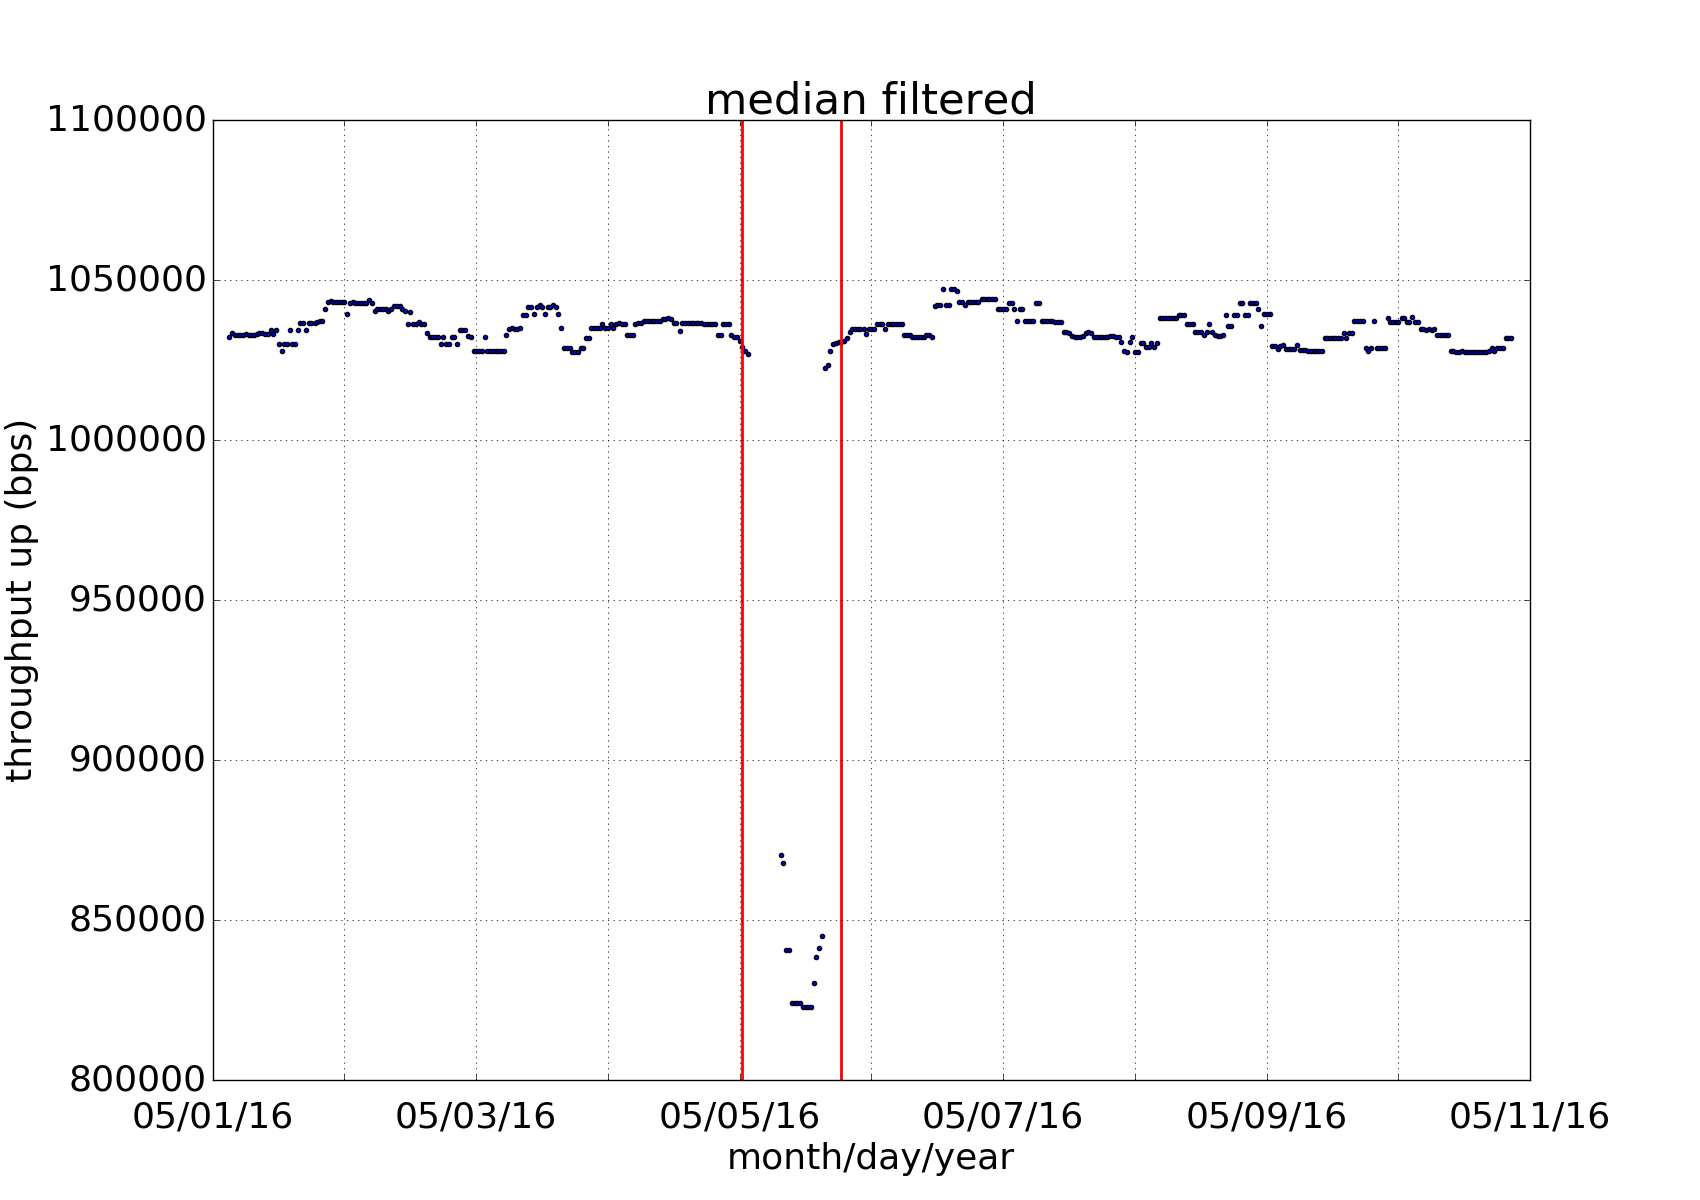
\includegraphics[width=\textwidth]{./figures/results/correct_examples/before_first_hop/serverSDRDTCLDM012_mac64:66:B3:50:06:D4_dtstart2016-05-01_dtend2016-05-11.png}
            \caption{Client 1.}
        \end{subfigure}
        \begin{subfigure}[b]{0.5\textwidth}
            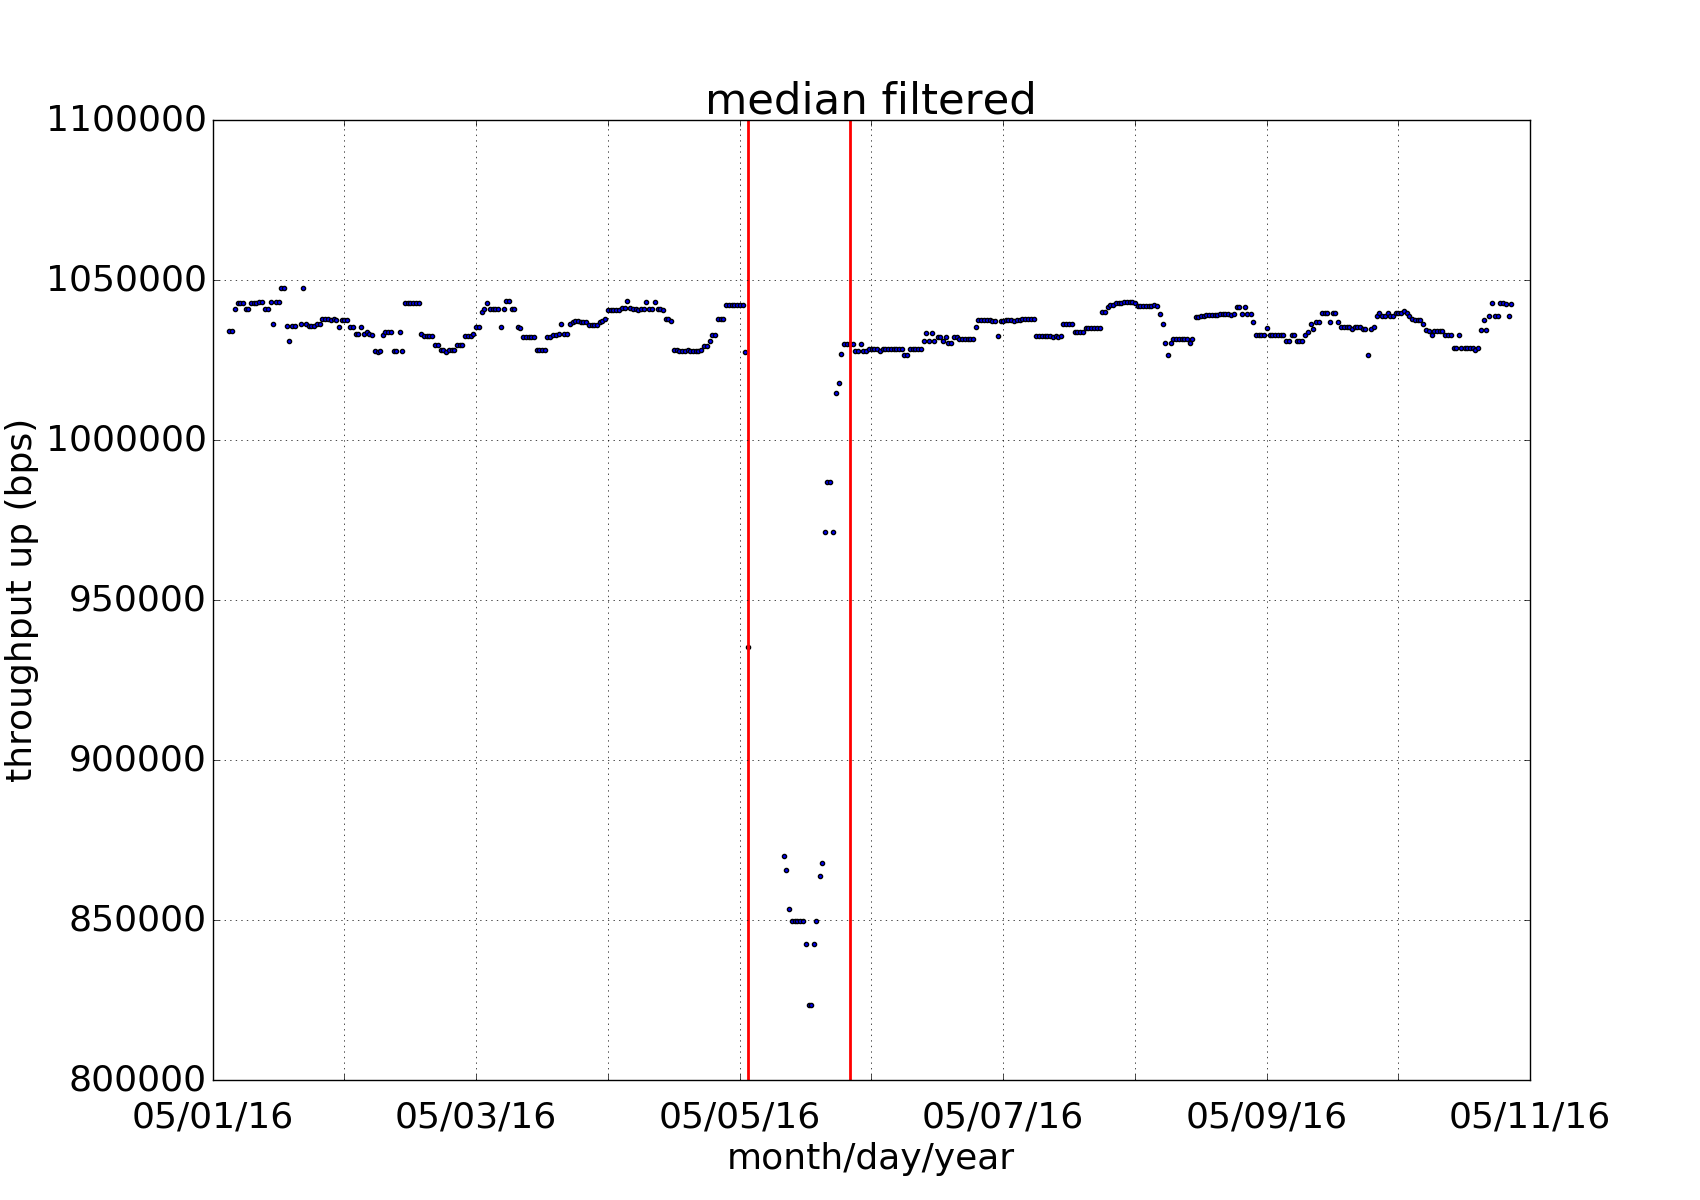
\includegraphics[width=\textwidth]{./figures/results/correct_examples/before_first_hop/serverSDRDTCLDM012_mac64:66:B3:A6:A9:70_dtstart2016-05-01_dtend2016-05-11.png}
            \caption{Client 2.}
        \end{subfigure}%
    }
    \caption{Before first hop.}
\label{fig:before_first_hop}
\end{figure}%

The system identified a network event at time X, in which only 2 of 4 clients
of the associated zero in degree vertex
clients perceived the event. Therefore, by the estabilished suppositions, they
share a physical equipment before the first hop, that caused this event.

\begin{figure}[H]
    \centering
    \makebox[\textwidth][c]{%
        \begin{subfigure}[b]{0.65\textwidth}
            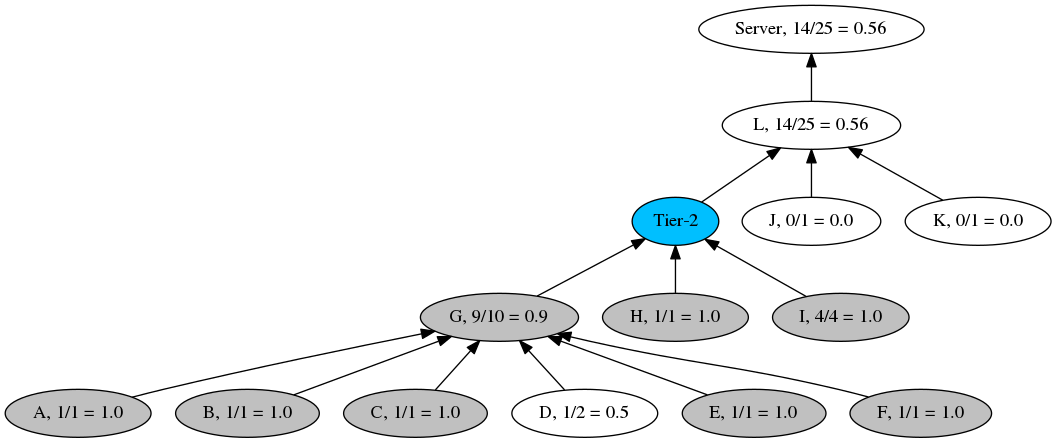
\includegraphics[width=\textwidth]{./figures/results/correct_examples/zero_indegree_correlation/dtstart2016-06-01_dtend2016-06-11_SOCDTCPEV01_traceroute_compress_embratel_graph_anonymized.png}
            \caption{Topology.}
        \end{subfigure}
        \begin{subfigure}[b]{0.45\textwidth}
            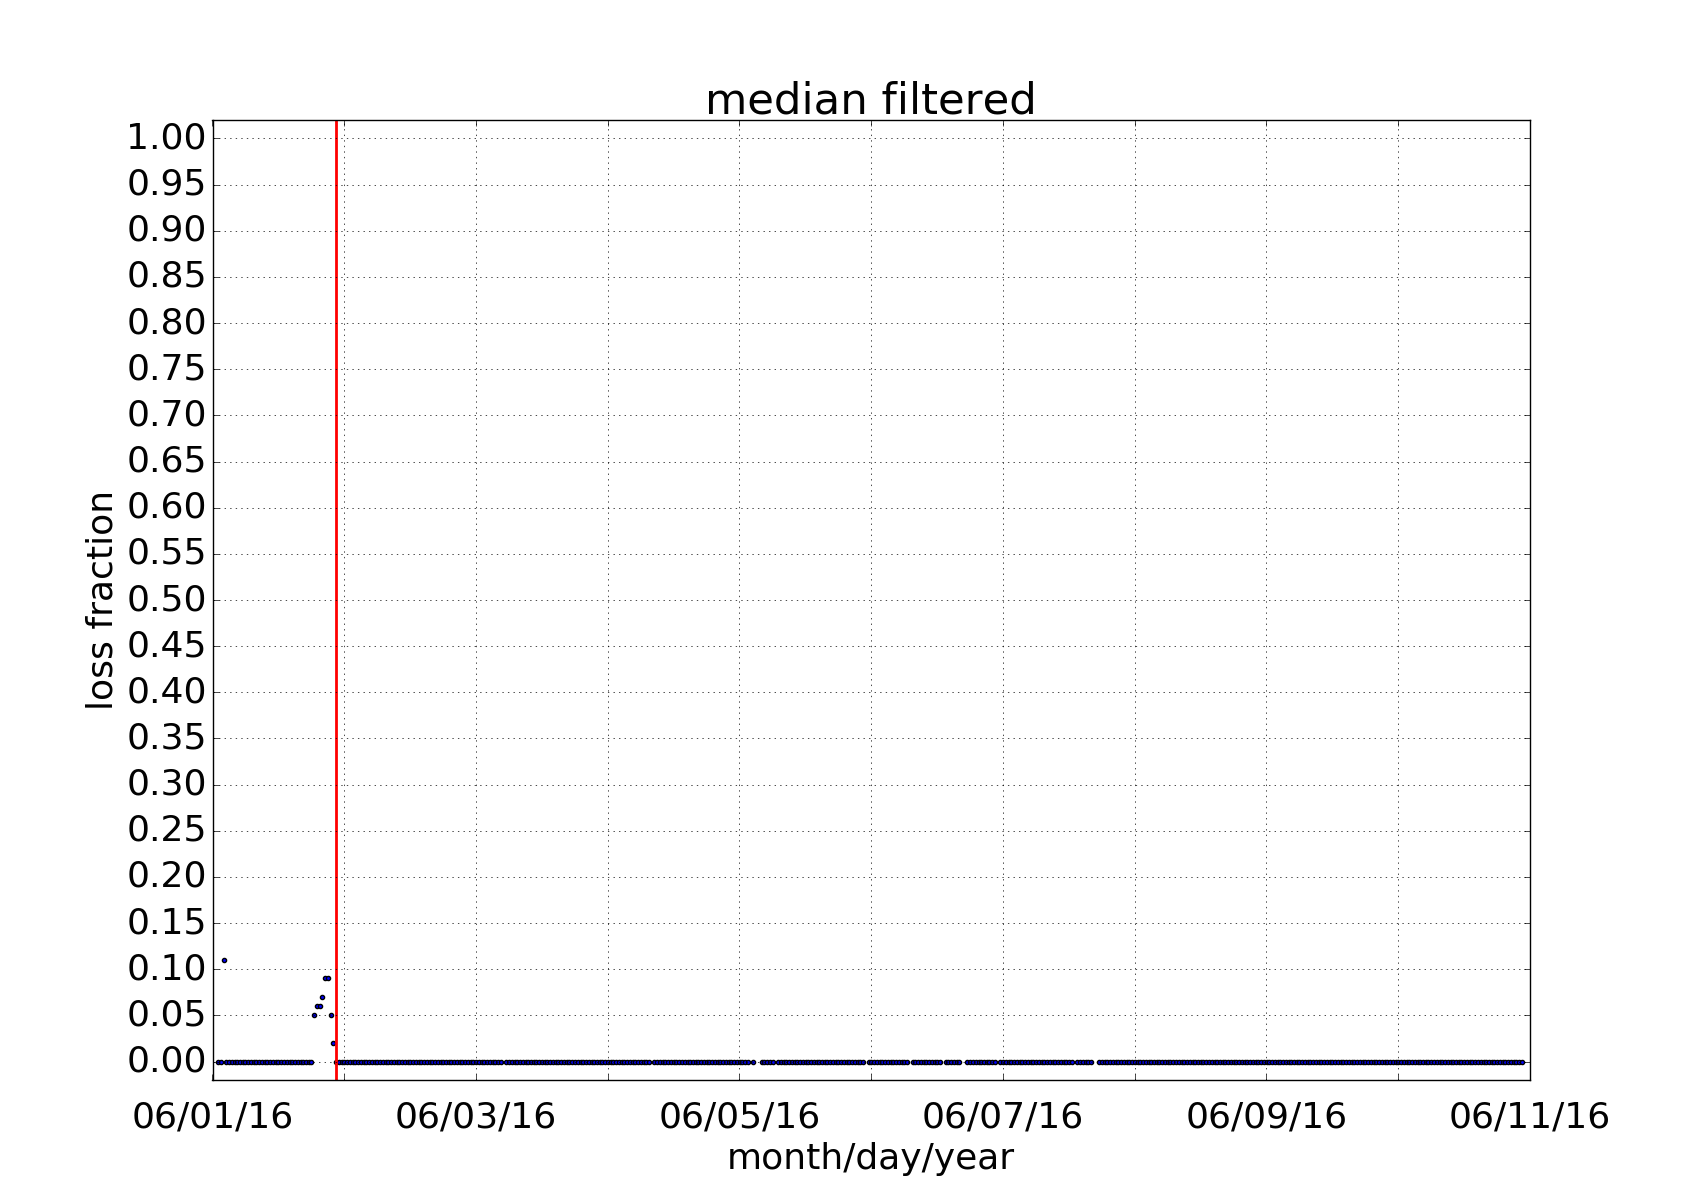
\includegraphics[width=\textwidth]{./figures/results/correct_examples/zero_indegree_correlation/serverSOCDTCPEV01_mac64:66:B3:4F:EA:E2_dtstart2016-06-01_dtend2016-06-11.png}
            \caption{Client 1.}
        \end{subfigure}%
    }
    \caption{Zero indegree correlation.}
\label{fig:zero_indegreee_correlation}
\end{figure}%

\begin{figure}[H]
    \centering
    \makebox[\textwidth][c]{%
        \begin{subfigure}[b]{0.65\textwidth}
            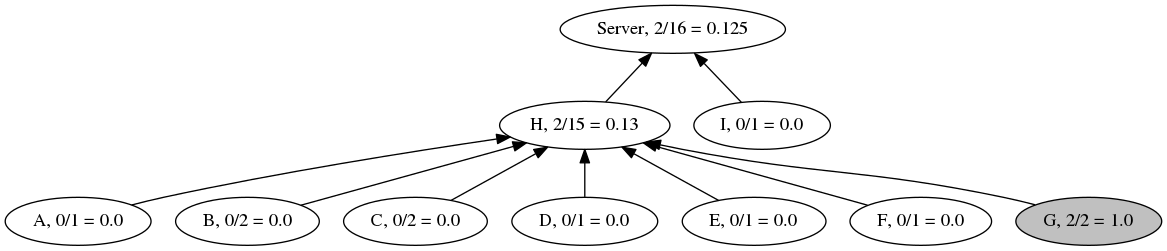
\includegraphics[width=\textwidth]{./figures/results/correct_examples/zero_indegree_single/dtstart2016-06-21_dtend2016-07-01_GRSCBCSRV01_traceroute_compress_embratel_filter_graph_anonymized.png}
            \caption{Topology.}
        \end{subfigure}
        \begin{subfigure}[b]{0.45\textwidth}
            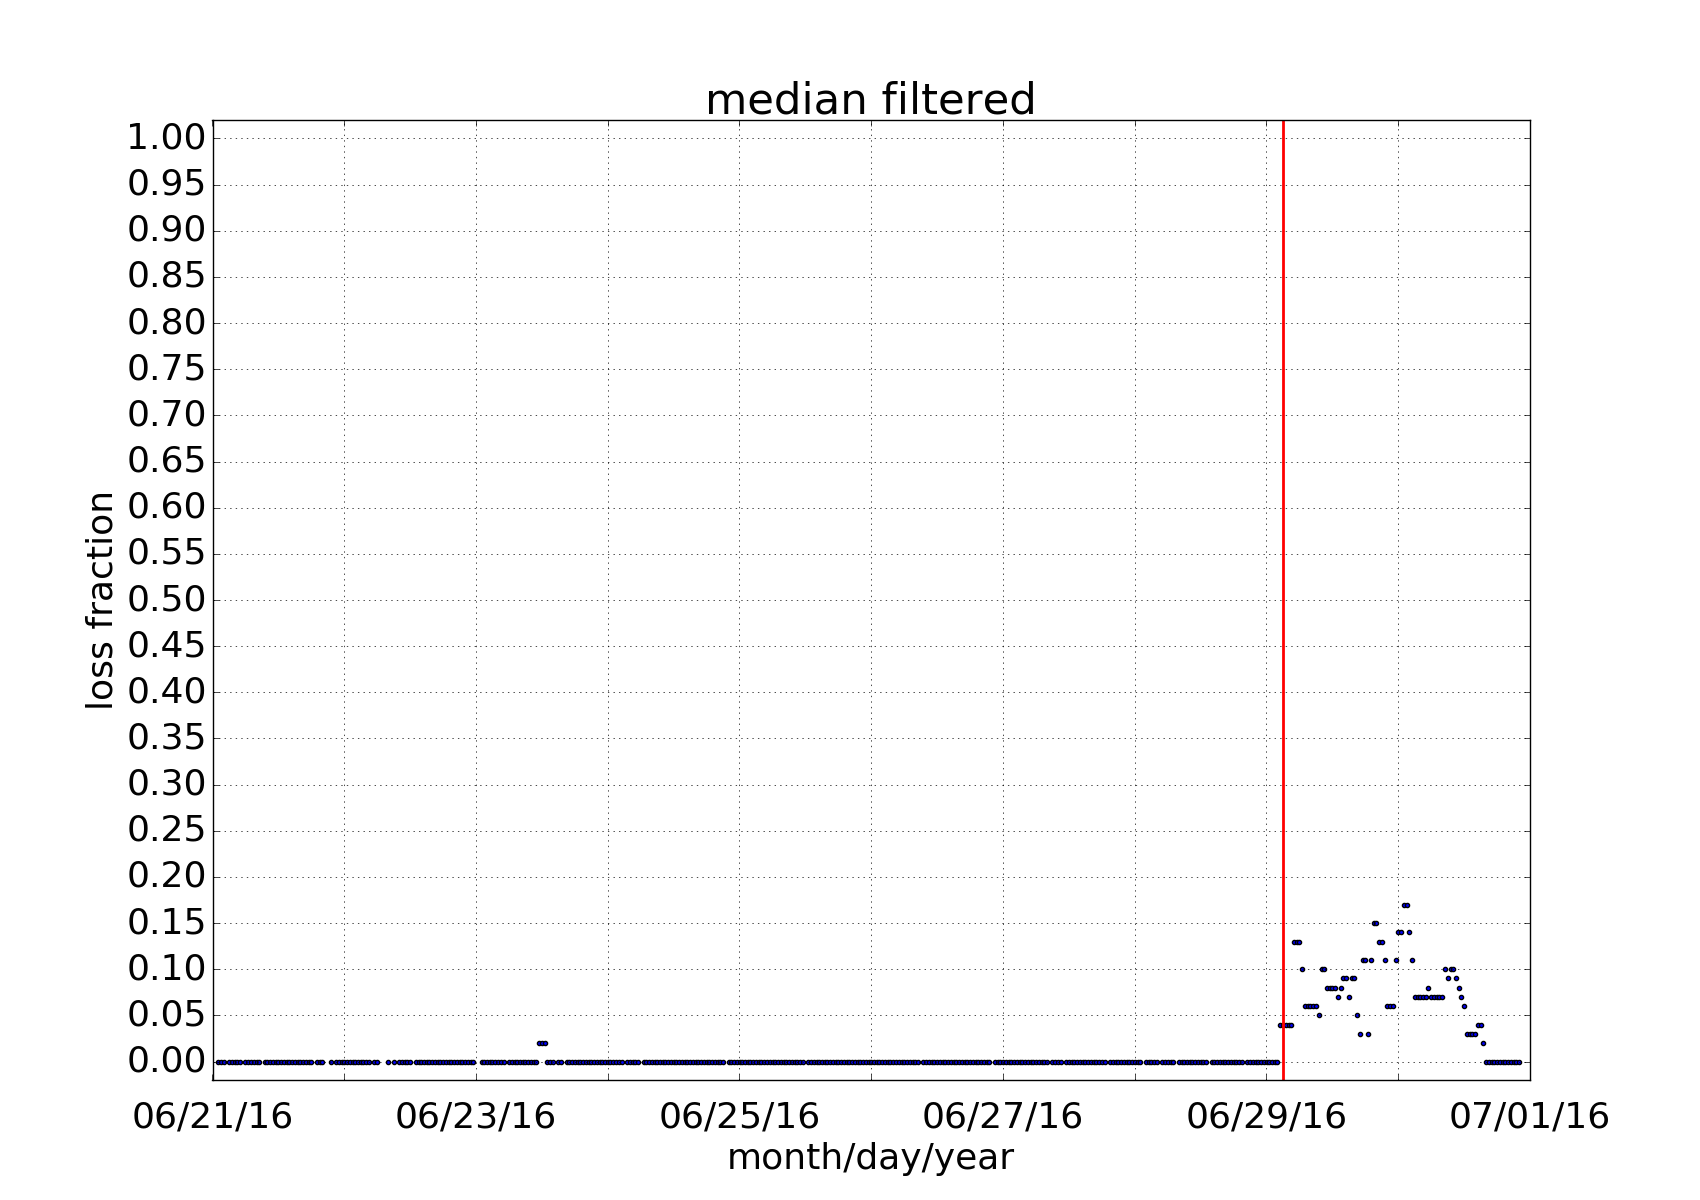
\includegraphics[width=\textwidth]{./figures/results/correct_examples/zero_indegree_single/serverGRSCBCSRV01_mac64:66:B3:50:05:56_dtstart2016-06-21_dtend2016-07-01.png}
            \caption{Client 1.}
        \end{subfigure}%
    }
    \caption{Zero indegree path analysis.}
\label{fig:zero_indegreee_without_correlation}
\end{figure}%

\section{Possible False Negative Examples}
\label{sec:possible_false_negative_examples}

17 clients with this pattern

\begin{figure}[H]
    \centering
    \makebox[\textwidth][c]{%
        \begin{subfigure}[b]{0.5\textwidth}
            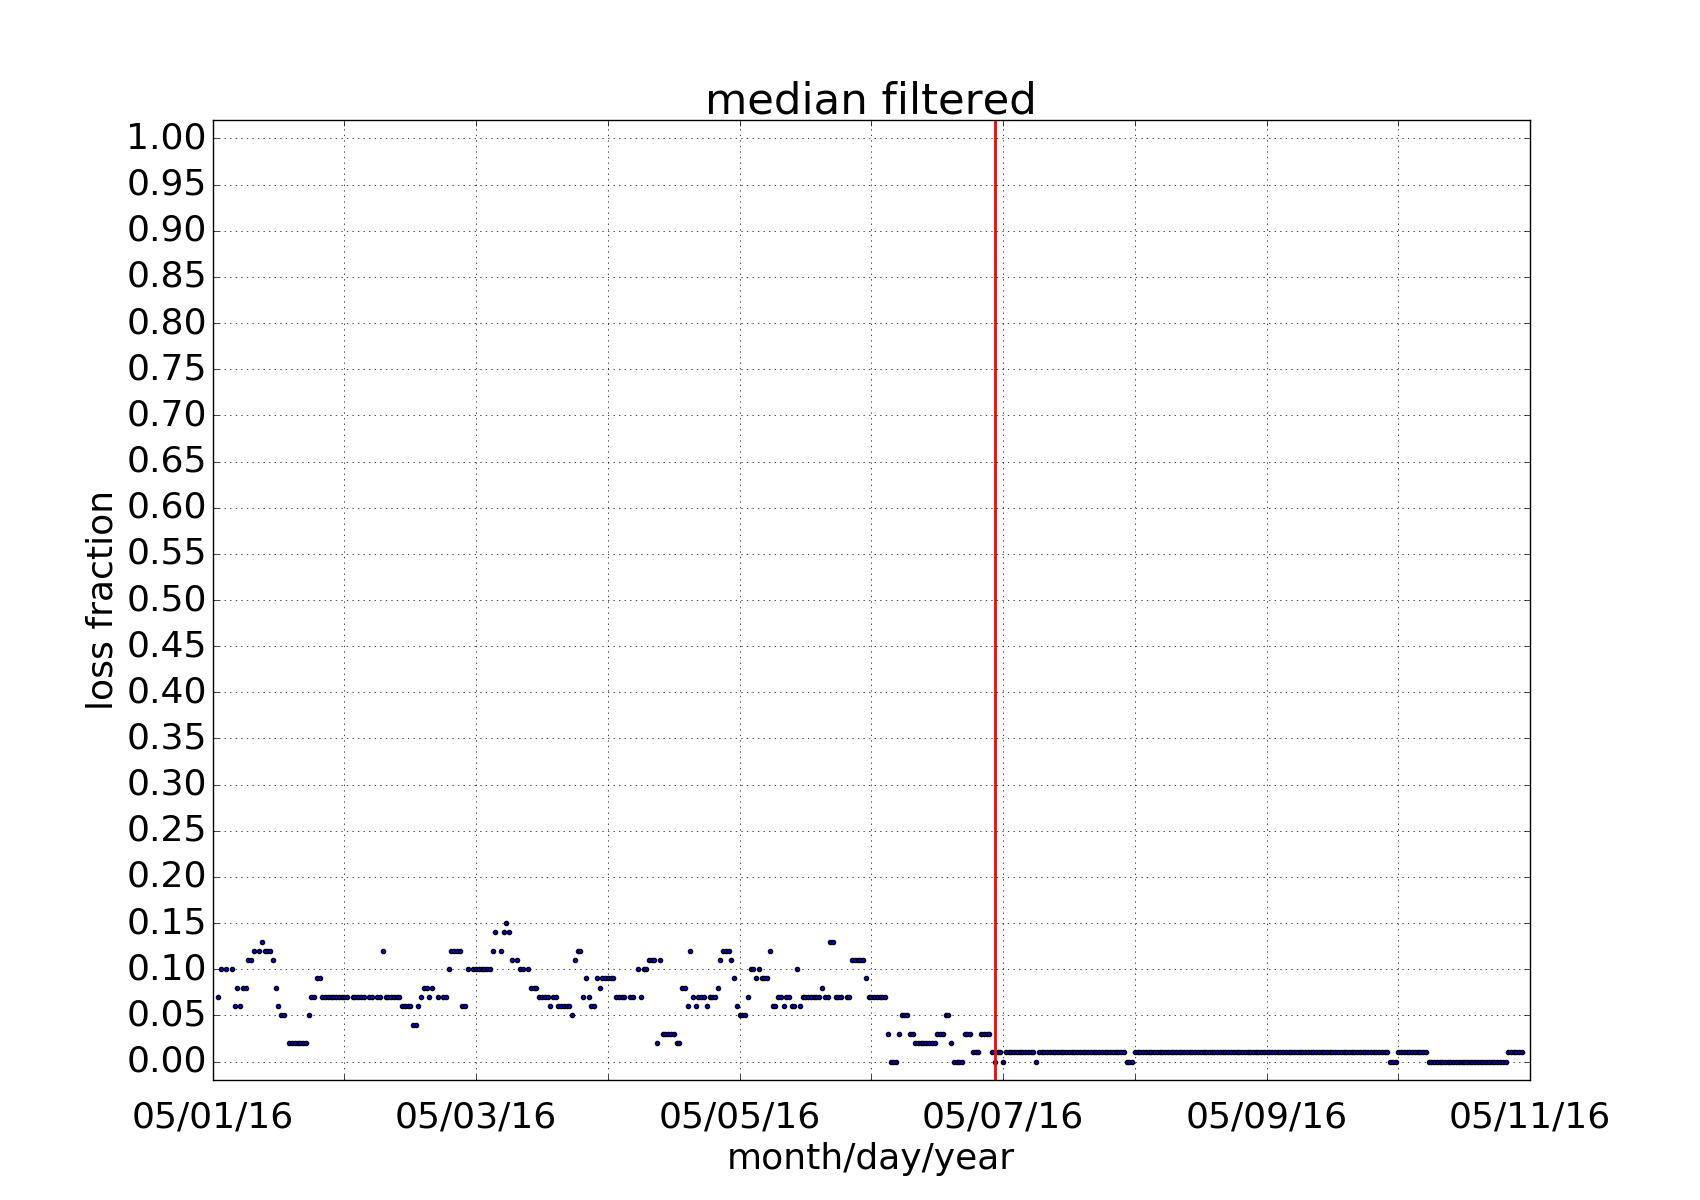
\includegraphics[width=\textwidth]{./figures/results/wrong_examples/time_correlation_example/serverSPOTVTSRV16_mac64:66:B3:A6:AB:80_dtstart2016-05-01_dtend2016-05-11.png}
            \caption{Client 1.}
        \end{subfigure}
        \begin{subfigure}[b]{0.5\textwidth}
            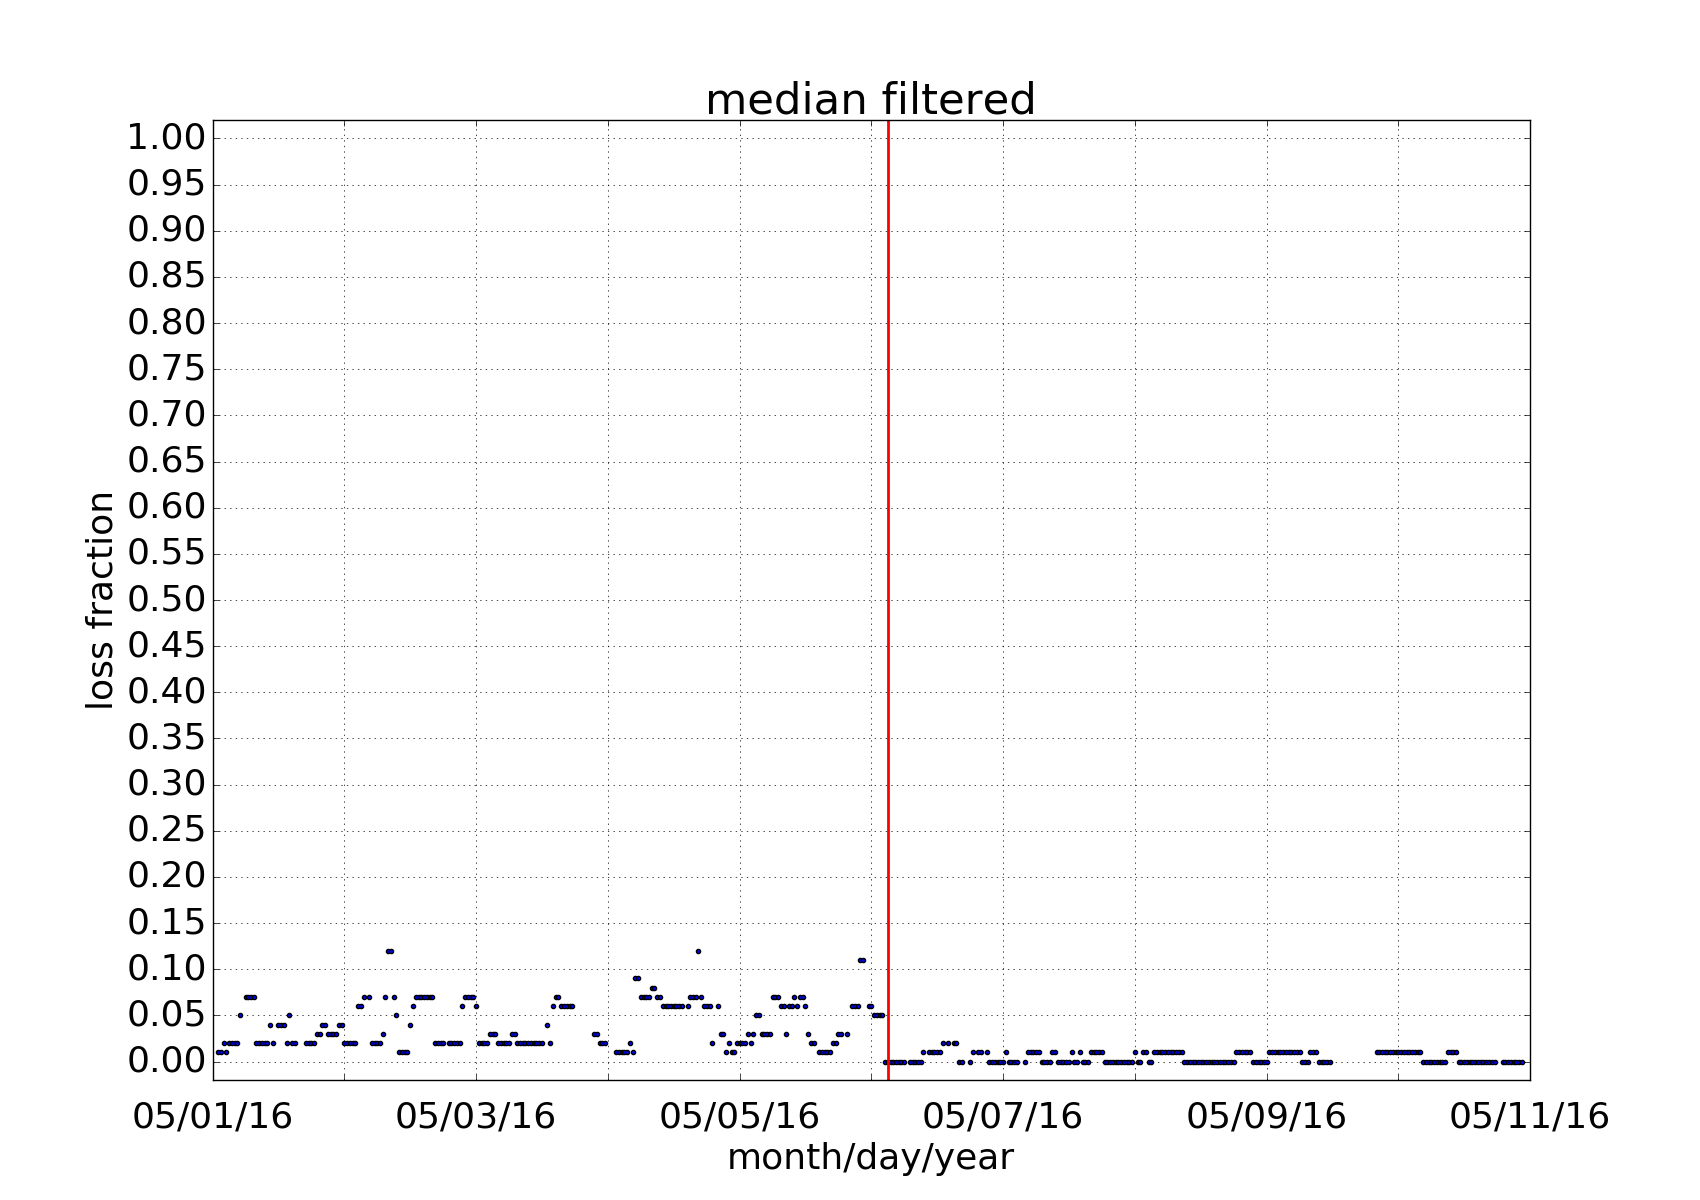
\includegraphics[width=\textwidth]{./figures/results/wrong_examples/time_correlation_example/serverSPOTVTSRV16_mac64:66:B3:A6:AC:40_dtstart2016-05-01_dtend2016-05-11.png}
            \caption{Client 2.}
        \end{subfigure}%
    }
    \caption{Untraceable location.}
\label{fig:untraceable_location}
\end{figure}%

\section{Events Without Traceable Location}
\label{sec:events_without_traceable_location}

In this example the traffic of the clients does'nt go to the Tier-2 ISP.

\begin{figure}[H]
    \centering
    \makebox[\textwidth][c]{%
        \begin{subfigure}[b]{0.5\textwidth}
            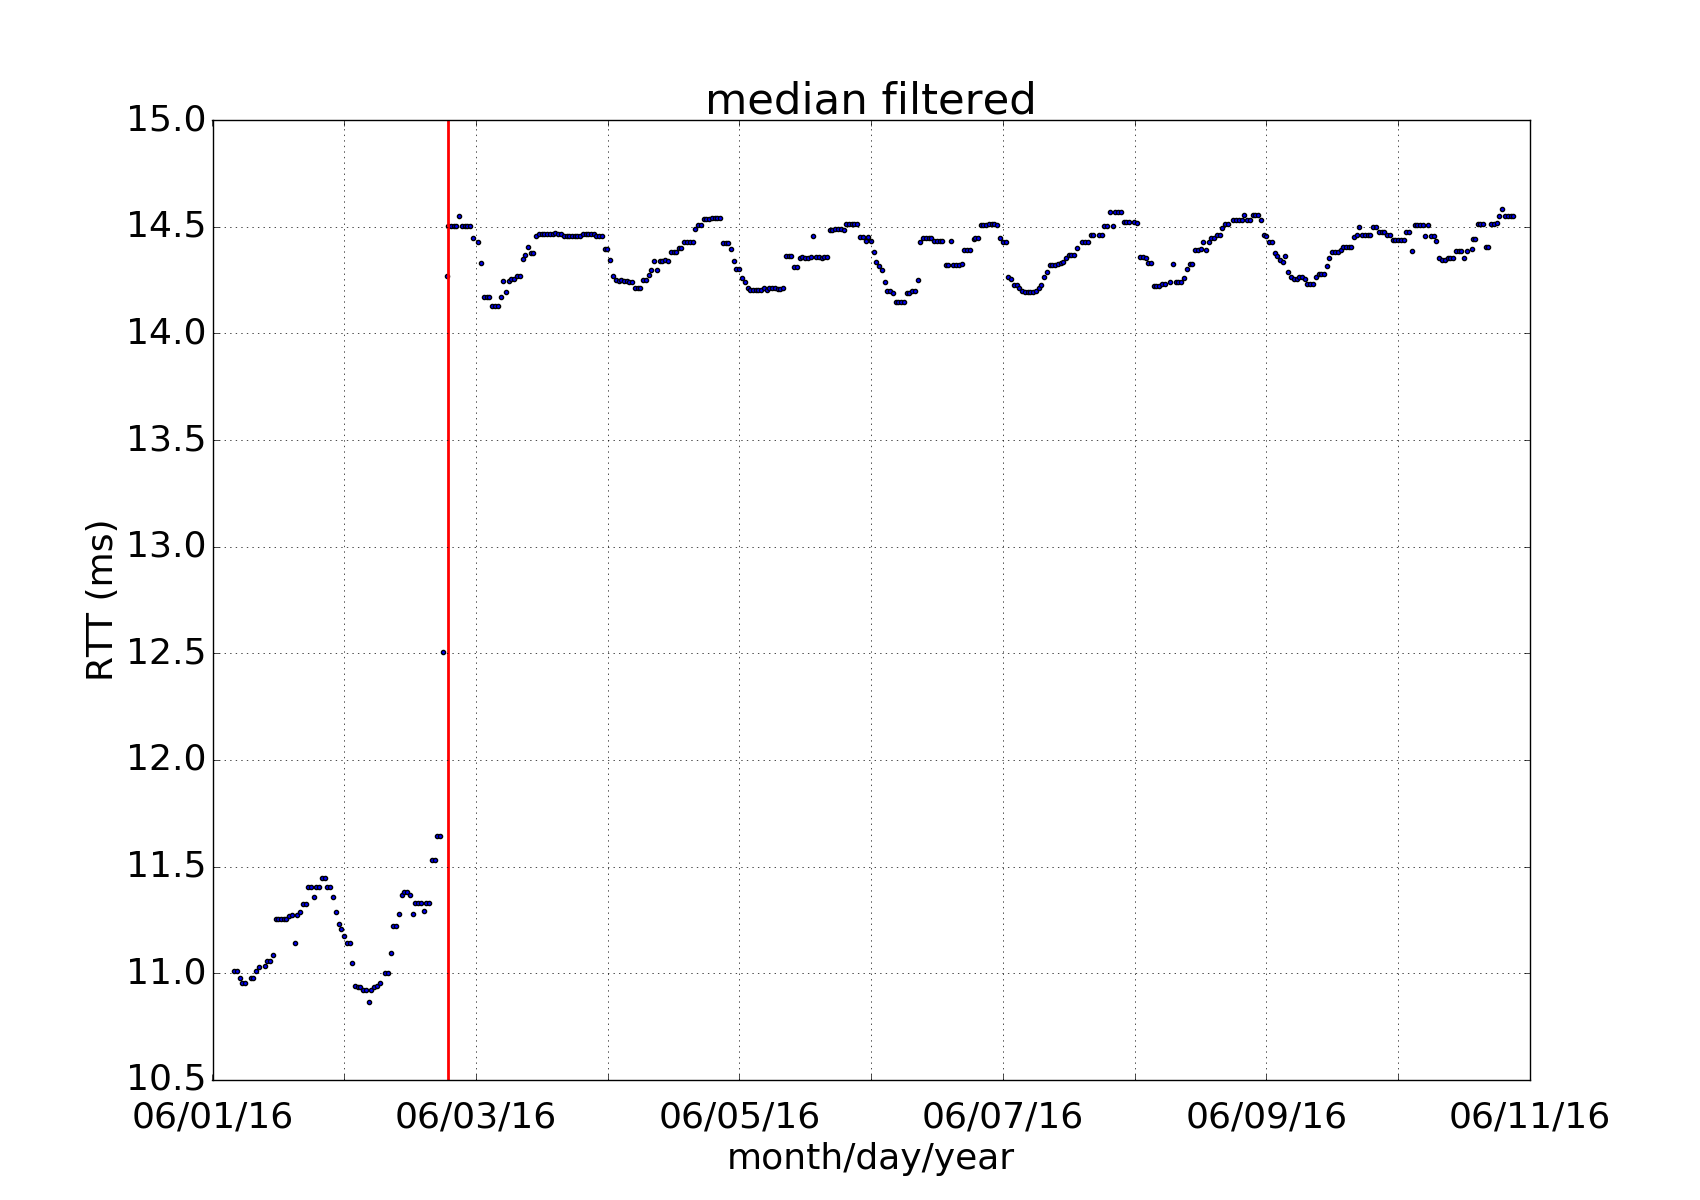
\includegraphics[width=\textwidth]{./figures/results/wrong_examples/untraceable_example/serverBHZDTCLDM062_mac64:66:B3:50:00:68_dtstart2016-06-01_dtend2016-06-11.png}
            \caption{Client 1.}
        \end{subfigure}
        \begin{subfigure}[b]{0.5\textwidth}
            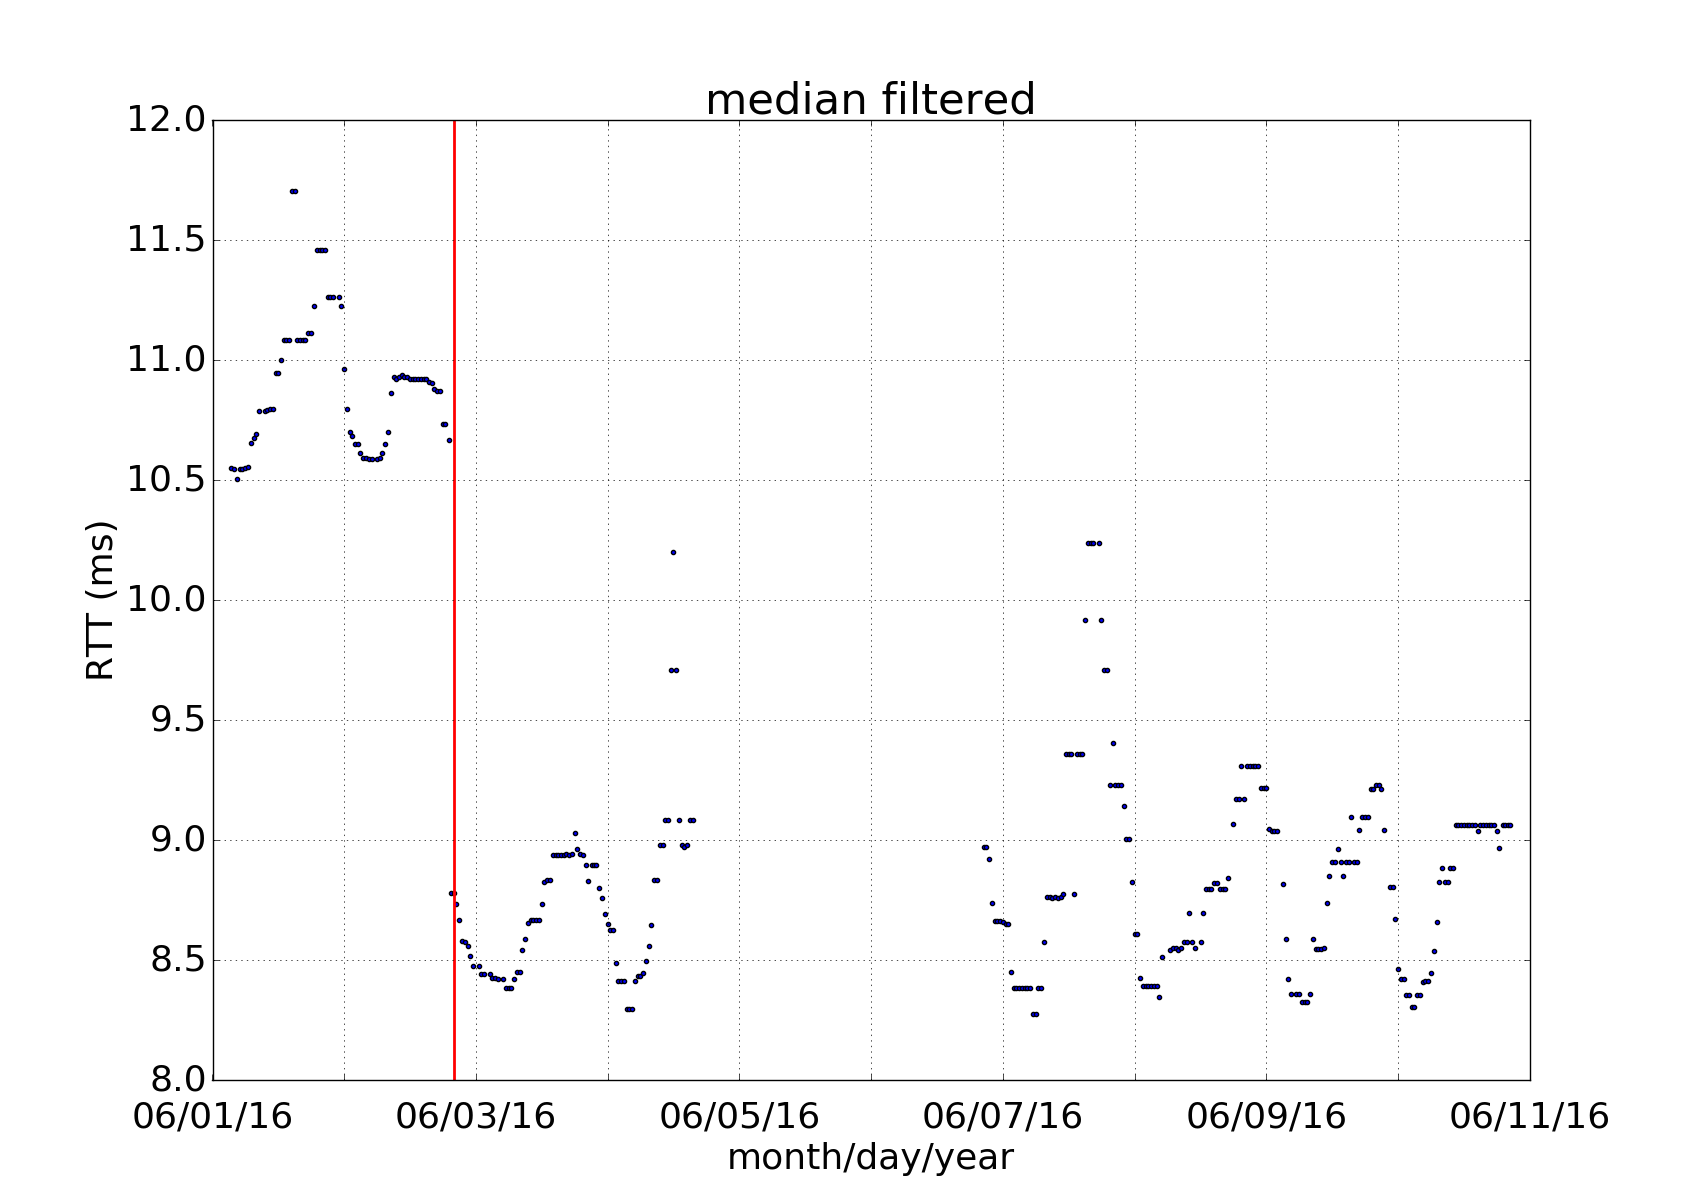
\includegraphics[width=\textwidth]{./figures/results/wrong_examples/untraceable_example/serverBHZDTCLDM062_mac64:66:B3:50:00:B6_dtstart2016-06-01_dtend2016-06-11.png}
            \caption{Client 2.}
        \end{subfigure}%
    }
    \caption{Untraceable location.}
\label{fig:untraceable_location}
\end{figure}%
